\documentclass[11pt]{article}
\usepackage[margin=1in]{geometry}
\usepackage{amsmath}
\usepackage{graphicx}
\usepackage{float}
\usepackage{longtable}
\usepackage{verbatim}
\title{Mandelbrot Float Renderer Benchmark Report}
\begin{document}
\maketitle

\section*{Method}
This report benchmarks the CPU renderers with a fixed scene centered at
(-0.743643887037151, 0.131825904205330) and zoom 180.0. Each configuration runs
5 times, with 40 warmup frames and 240
measured frames per run. Single-threaded variants are pinned to CPU list
\texttt{3}; the threaded renderer is pinned to
\texttt{0-15}. Telemetry is sampled every
0.50 seconds, with a configured cooldown of
0.0 seconds between runs.
The benchmark shell requested governor {performance}
before running the measurements.

Representative data requires at least 5 runs, matching
checksums, at least 60 measured frames per run,
no thermal-throttle counter increments, and a between-run coefficient of variation no higher than
5.0\%.

\section*{Summary Table}
\subsection*{CPU Compute}
\begin{longtable}{llllrrrrll}
Opt & Variant & Mean ms & Std ms & CV \% & Base \% & Prev \% & RSS MiB & Rep & Match \\ \hline
\endfirsthead
Opt & Variant & Mean ms & Std ms & CV \% & Base \% & Prev \% & RSS MiB & Rep & Match \\ \hline
\endhead
-O1 & naive & 106.900 & 0.224 & 0.21 & +0.0 & -- & 19.69 & yes & yes \\
-O1 & arrays & 498.299 & 12.810 & 2.57 & -366.1 & -366.1 & 19.94 & no & no \\
-O1 & simd & 100.786 & 0.603 & 0.60 & +5.7 & +79.8 & 19.94 & yes & no \\
-O1 & simd\_threads & 11.729 & 0.044 & 0.37 & +89.0 & +88.4 & 19.94 & yes & no \\
-O2 & naive & 99.707 & 0.575 & 0.58 & +0.0 & -- & 19.94 & yes & yes \\
-O2 & arrays & 107.651 & 0.283 & 0.26 & -8.0 & -8.0 & 19.94 & yes & no \\
-O2 & simd & 48.462 & 0.211 & 0.43 & +51.4 & +55.0 & 19.94 & yes & no \\
-O2 & simd\_threads & 10.570 & 0.034 & 0.32 & +89.4 & +78.2 & 19.94 & yes & no \\
-O3 & naive & 100.314 & 1.441 & 1.44 & +0.0 & -- & 19.94 & yes & yes \\
-O3 & arrays & 56.826 & 0.137 & 0.24 & +43.4 & +43.4 & 19.94 & yes & no \\
-O3 & simd & 49.283 & 0.259 & 0.53 & +50.9 & +13.3 & 19.94 & yes & no \\
-O3 & simd\_threads & 10.633 & 0.052 & 0.49 & +89.4 & +78.4 & 19.94 & yes & no \\
\end{longtable}

\subsection*{Hidden-Window Presentation}
\begin{longtable}{lrrrrr}
Variant & n & Render ms & Present ms & Total ms & Present \% total \\ \hline
\endfirsthead
Variant & n & Render ms & Present ms & Total ms & Present \% total \\ \hline
\endhead
naive & 2 & 230.530 & 1.671 & 232.201 & 0.72 \\
arrays & 2 & 127.401 & 1.614 & 129.015 & 1.25 \\
simd & 2 & 112.570 & 1.632 & 114.202 & 1.43 \\
simd\_threads & 2 & 10.456 & 1.630 & 12.086 & 13.49 \\
\end{longtable}

\subsection*{GPU Render}
\begin{longtable}{lrr}
Variant & n & Render ms \\ \hline
\endfirsthead
Variant & n & Render ms \\ \hline
\endhead
gpu & 3 & 7.507 \\
\end{longtable}

\section*{Uncertainty}
Repeated-run uncertainty is reported for CPU, hidden-window, and GPU measurements using:
\[
\sigma = \sqrt{\frac{1}{n - 1} \sum_{i=1}^{n} (x_i - \bar{x})^2}
\]
\[
\mathrm{SEM} = \frac{\sigma}{\sqrt{n}}, \quad
\mathrm{CI}_{95} = t_{0.975, n-1} \cdot \frac{\sigma}{\sqrt{n}}, \quad
\mathrm{Inacc.\%} = 100 \cdot \frac{\mathrm{CI}_{95}}{\bar{x}}
\]

\subsection*{CPU Compute}
\begin{longtable}{lllrrrrrr}
Opt & Variant & n & Mean ms & $-\sigma$ ms & $+\sigma$ ms & SEM ms & 95\% $\pm$ ms & Inacc. \% \\ \hline
\endfirsthead
Opt & Variant & n & Mean ms & $-\sigma$ ms & $+\sigma$ ms & SEM ms & 95\% $\pm$ ms & Inacc. \% \\ \hline
\endhead
-O1 & naive & 5 & 106.900 & 106.675 & 107.124 & 0.100 & 0.279 & 0.26 \\
-O1 & arrays & 5 & 498.299 & 485.489 & 511.109 & 5.729 & 15.903 & 3.19 \\
-O1 & simd & 5 & 100.786 & 100.183 & 101.389 & 0.270 & 0.748 & 0.74 \\
-O1 & simd\_threads & 5 & 11.729 & 11.685 & 11.772 & 0.019 & 0.054 & 0.46 \\
-O2 & naive & 5 & 99.707 & 99.132 & 100.283 & 0.257 & 0.714 & 0.72 \\
-O2 & arrays & 5 & 107.651 & 107.367 & 107.934 & 0.127 & 0.352 & 0.33 \\
-O2 & simd & 5 & 48.462 & 48.252 & 48.673 & 0.094 & 0.261 & 0.54 \\
-O2 & simd\_threads & 5 & 10.570 & 10.536 & 10.604 & 0.015 & 0.042 & 0.40 \\
-O3 & naive & 5 & 100.314 & 98.873 & 101.755 & 0.644 & 1.789 & 1.78 \\
-O3 & arrays & 5 & 56.826 & 56.689 & 56.963 & 0.061 & 0.170 & 0.30 \\
-O3 & simd & 5 & 49.283 & 49.024 & 49.542 & 0.116 & 0.322 & 0.65 \\
-O3 & simd\_threads & 5 & 10.633 & 10.581 & 10.684 & 0.023 & 0.064 & 0.60 \\
\end{longtable}

\subsection*{Hidden-Window Presentation}
\begin{longtable}{llrrrrrrrr}
Variant & n & Render ms & $\sigma_R$ & Present ms & $\sigma_P$ & Total ms & $\sigma_T$ & 95\% $\pm_T$ & Inacc. \% \\ \hline
\endfirsthead
Variant & n & Render ms & $\sigma_R$ & Present ms & $\sigma_P$ & Total ms & $\sigma_T$ & 95\% $\pm_T$ & Inacc. \% \\ \hline
\endhead
naive & 2 & 230.530 & 0.701 & 1.671 & 0.058 & 232.201 & 0.759 & 6.816 & 2.94 \\
arrays & 2 & 127.401 & 0.077 & 1.614 & 0.002 & 129.015 & 0.079 & 0.709 & 0.55 \\
simd & 2 & 112.570 & 0.054 & 1.632 & 0.022 & 114.202 & 0.076 & 0.686 & 0.60 \\
simd\_threads & 2 & 10.456 & 0.096 & 1.630 & 0.048 & 12.086 & 0.144 & 1.293 & 10.70 \\
\end{longtable}

\subsection*{GPU Render}
\begin{longtable}{lrrrrrr}
Variant & n & Render ms & $\sigma_R$ & SEM ms & 95\% $\pm_R$ & Inacc. \% \\ \hline
\endfirsthead
Variant & n & Render ms & $\sigma_R$ & SEM ms & 95\% $\pm_R$ & Inacc. \% \\ \hline
\endhead
gpu & 3 & 7.507 & 0.249 & 0.144 & 0.619 & 8.24 \\
\end{longtable}

\section*{Environment}
\begin{verbatim}
analyzing CPU 7:
  current policy: frequency should be within 400 MHz and 4.50 GHz.
                  The governor "performance" may decide which speed to use
                  within this range.
\end{verbatim}
\begin{verbatim}
Architecture:                            x86_64
CPU op-mode(s):                          32-bit, 64-bit
Address sizes:                           46 bits physical, 48 bits virtual
Byte Order:                              Little Endian
CPU(s):                                  16
On-line CPU(s) list:                     0-15
Vendor ID:                               GenuineIntel
Model name:                              Intel(R) Core(TM) Ultra 9 285H
CPU family:                              6
Model:                                   197
Thread(s) per core:                      1
Core(s) per socket:                      16
Socket(s):                               1
Stepping:                                2
CPU(s) scaling MHz:                      69%
CPU max MHz:                             5400,0000
CPU min MHz:                             400,0000
BogoMIPS:                                7372,80
Virtualization:                          VT-x
L1d cache:                               480 KiB (12 instances)
L1i cache:                               768 KiB (12 instances)
L2 cache:                                28 MiB (9 instances)
L3 cache:                                24 MiB (1 instance)
\end{verbatim}

\section*{Plots}
\begin{figure}[H]
\centering
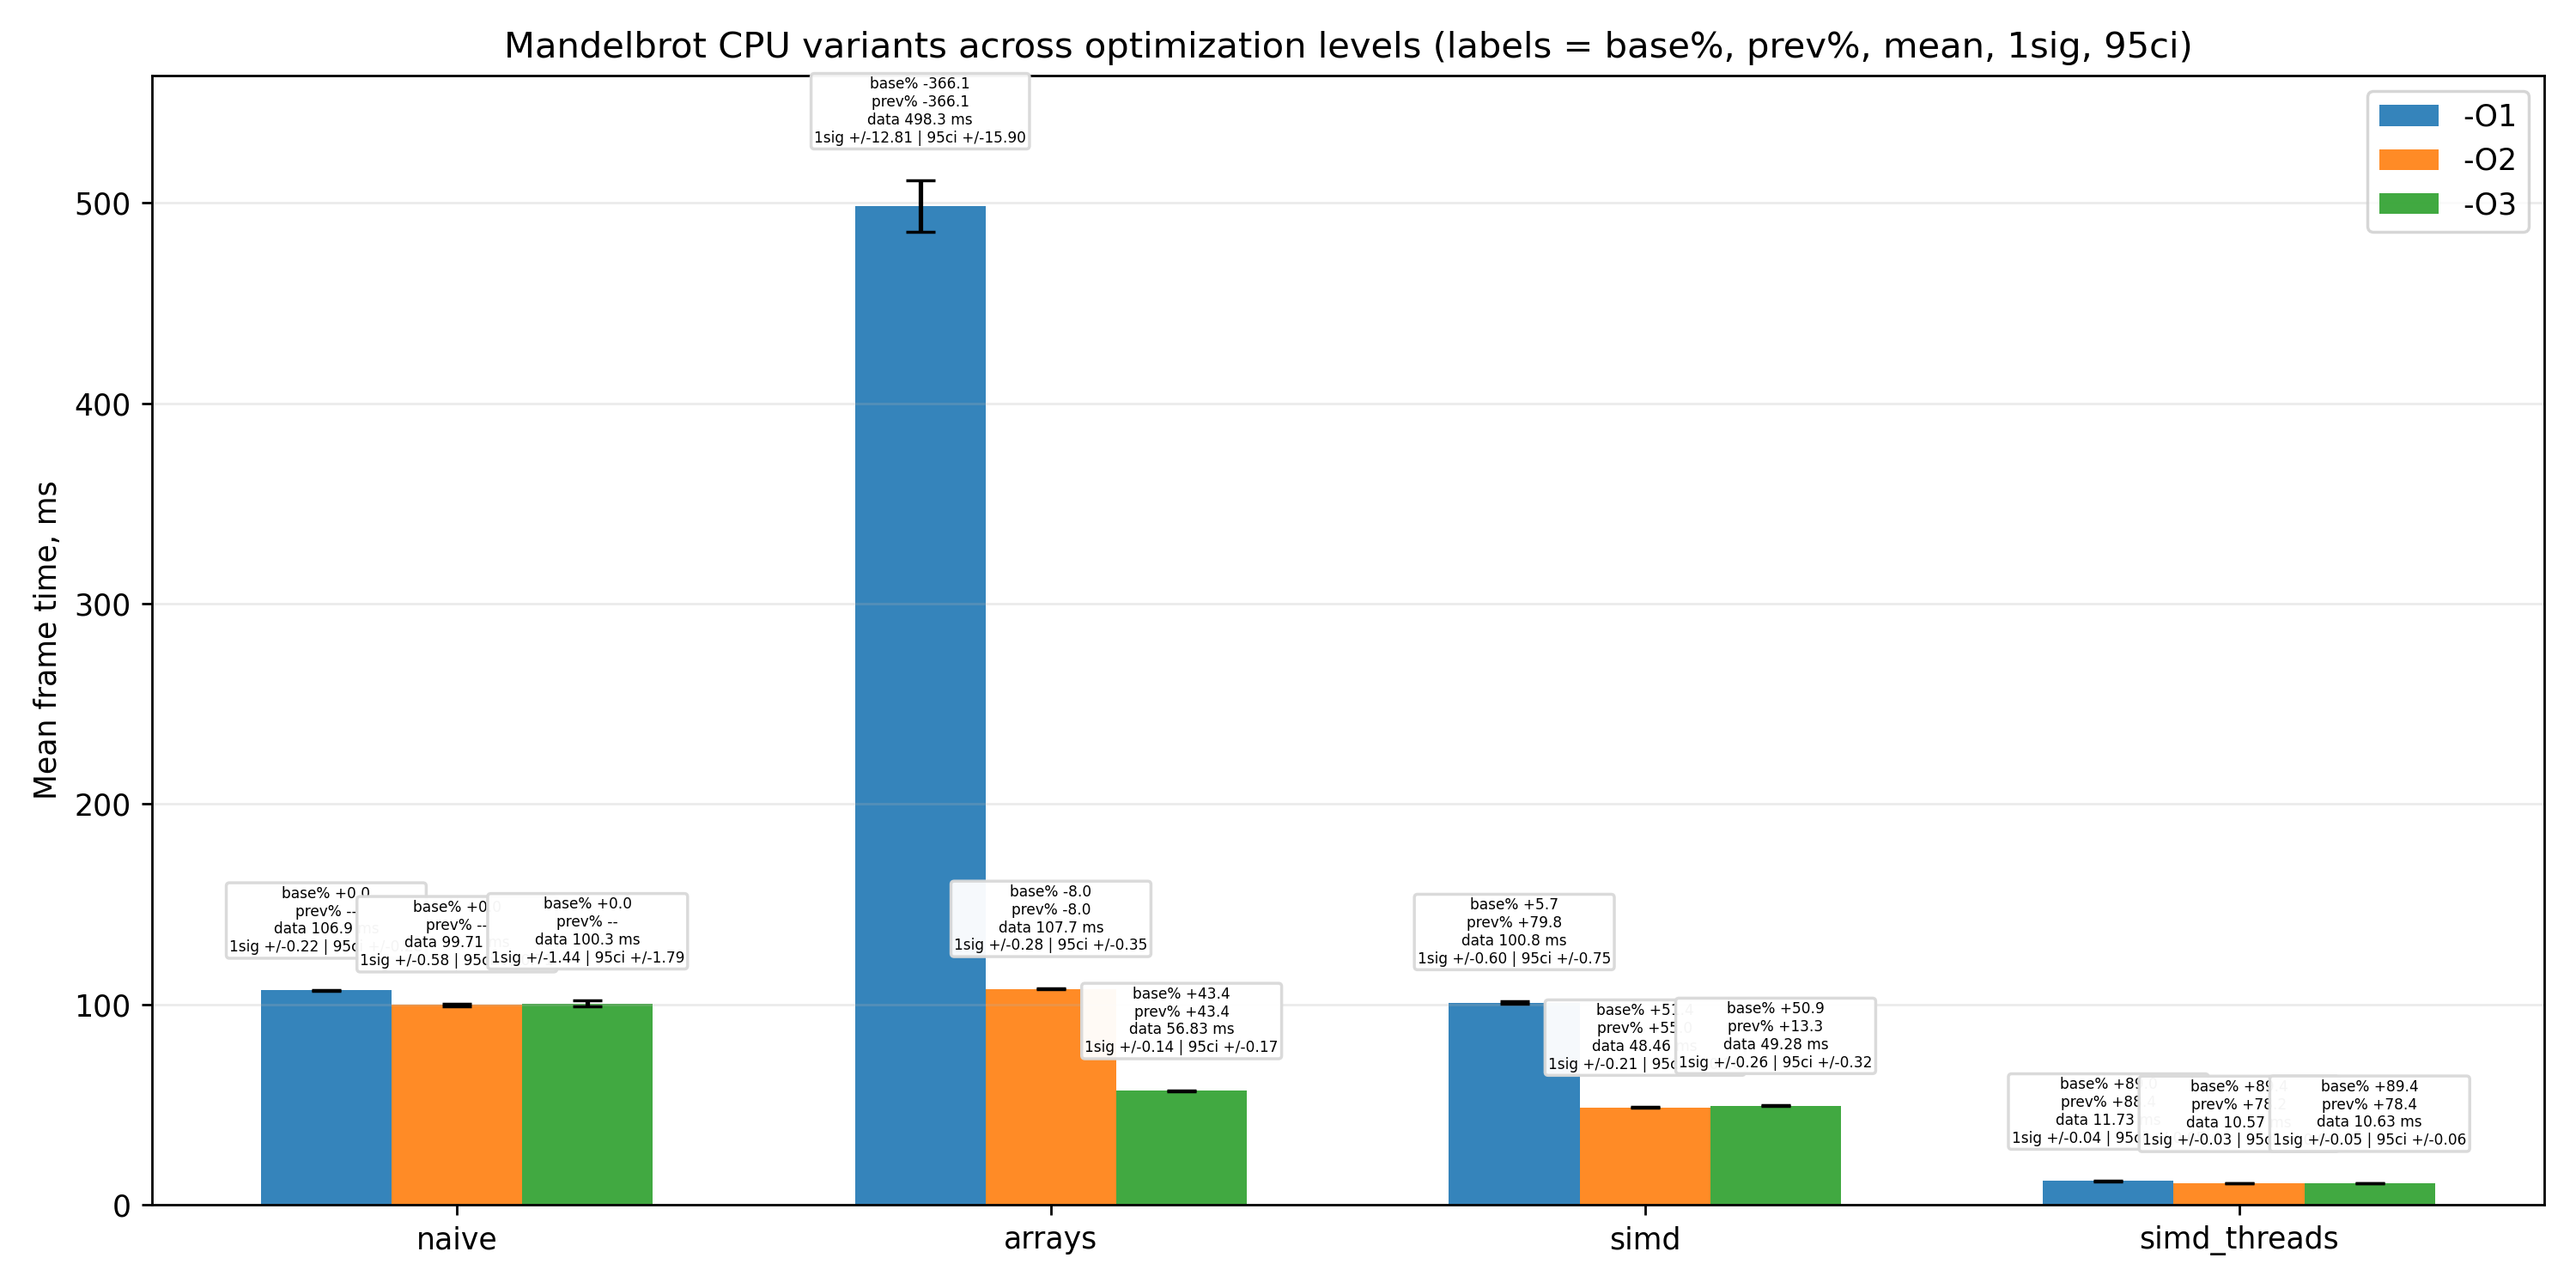
\includegraphics[width=0.95\linewidth]{../img/plots/benchmark_all_opts.png}
\end{figure}

\begin{figure}[H]
\centering
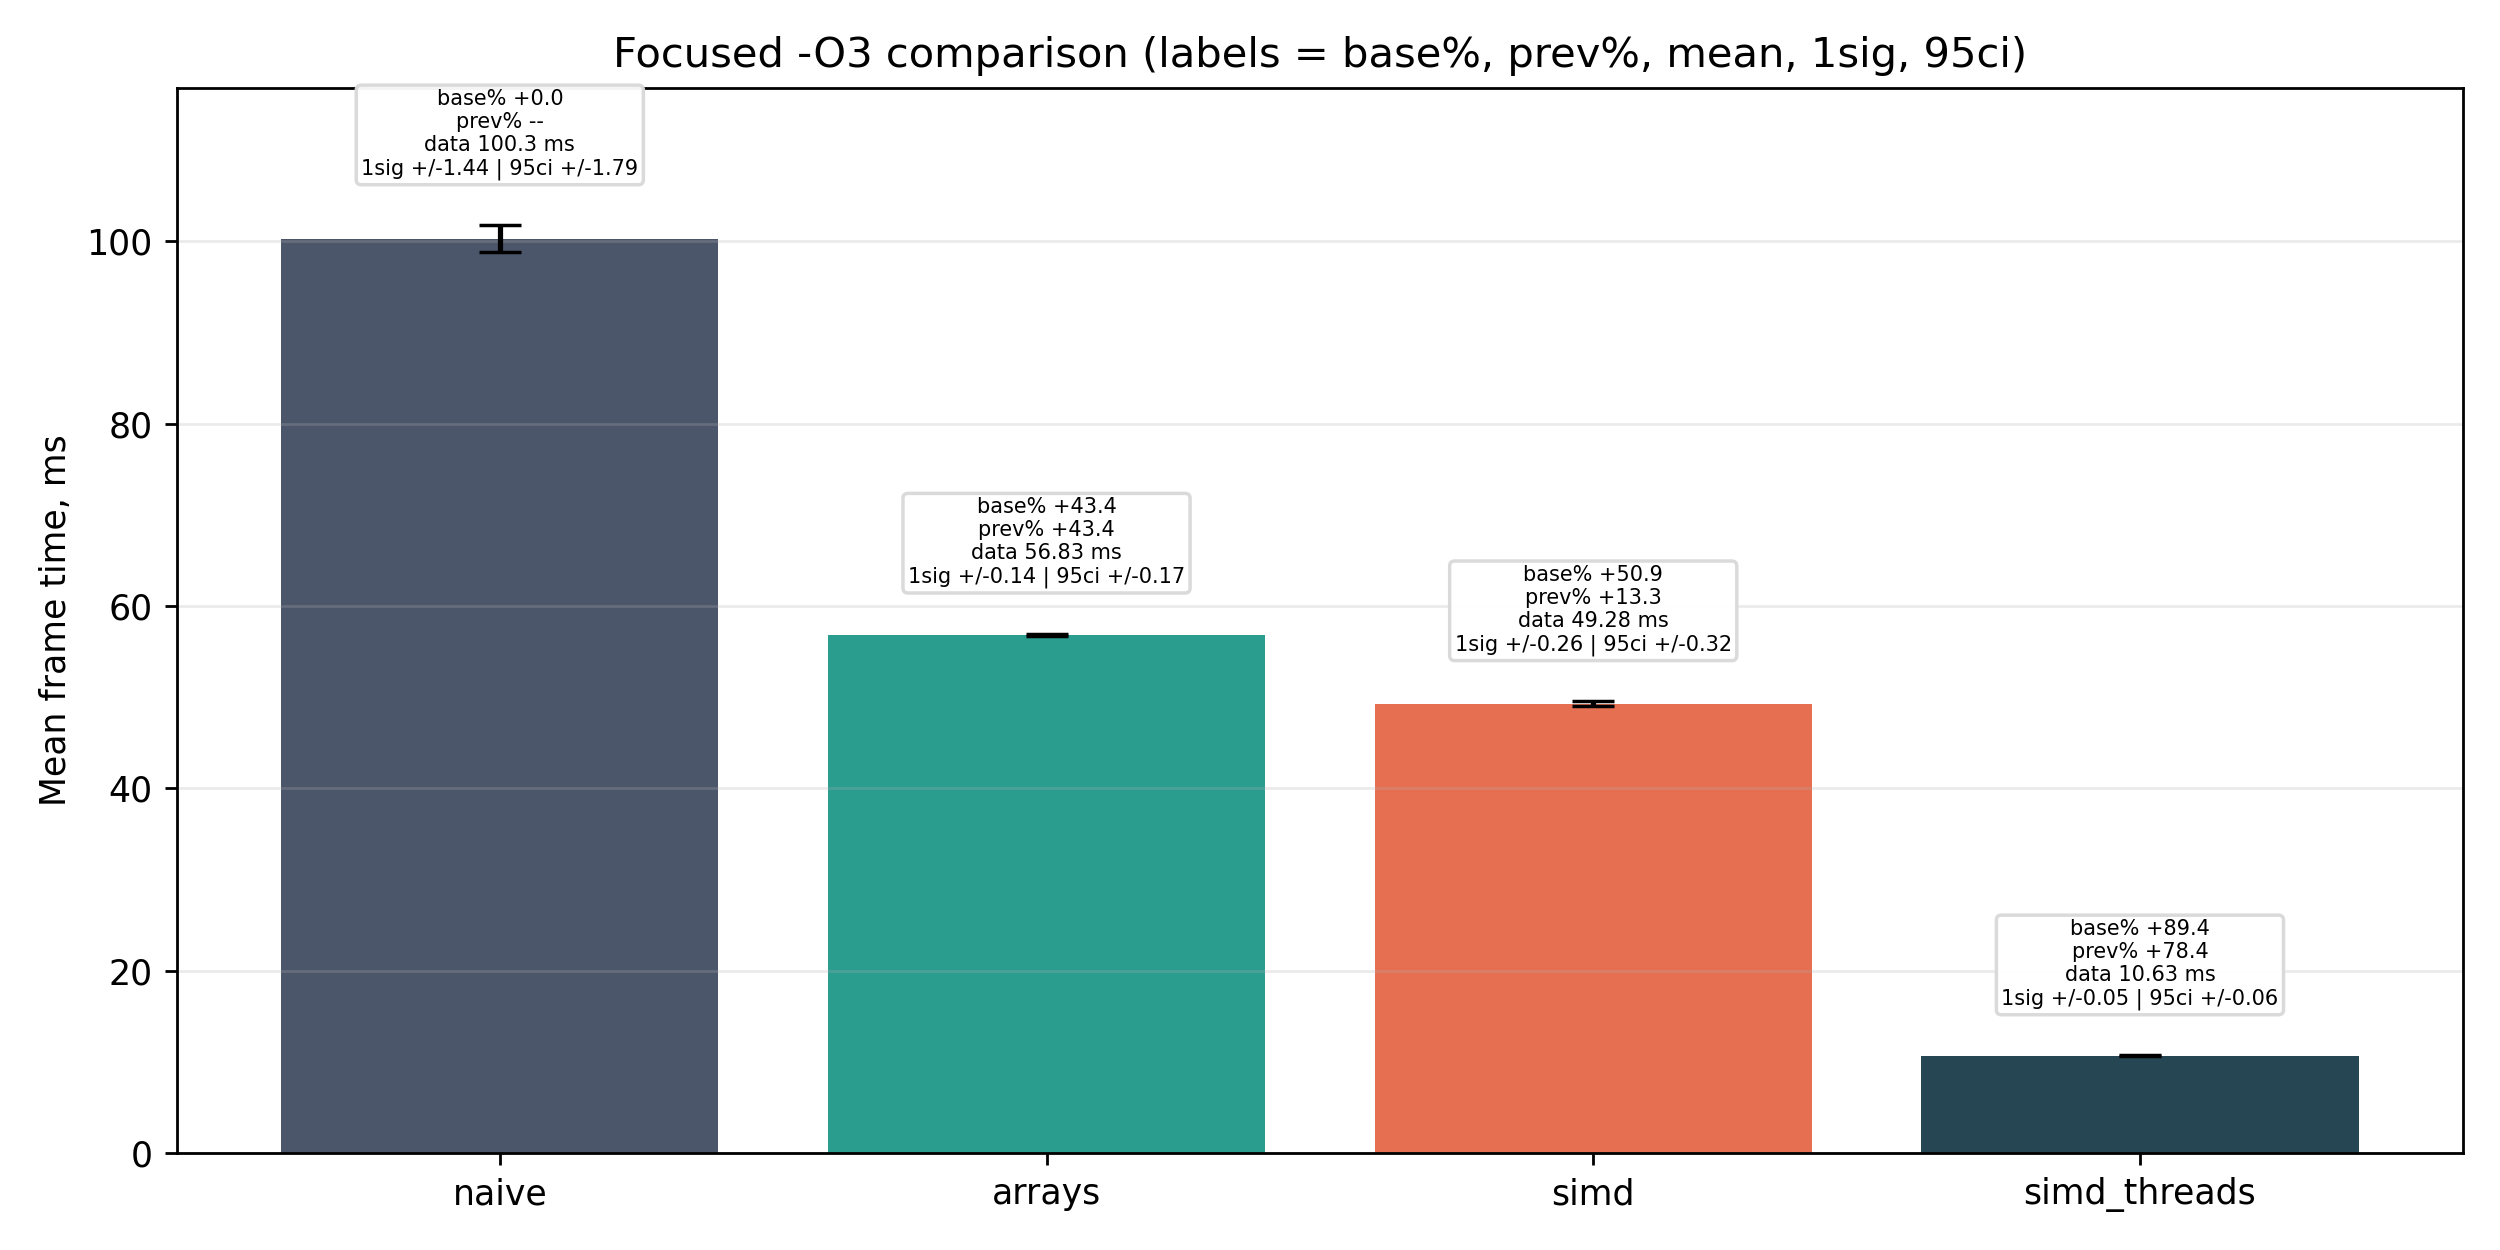
\includegraphics[width=0.95\linewidth]{../img/plots/benchmark_o3_focus.png}
\end{figure}

\begin{figure}[H]
\centering
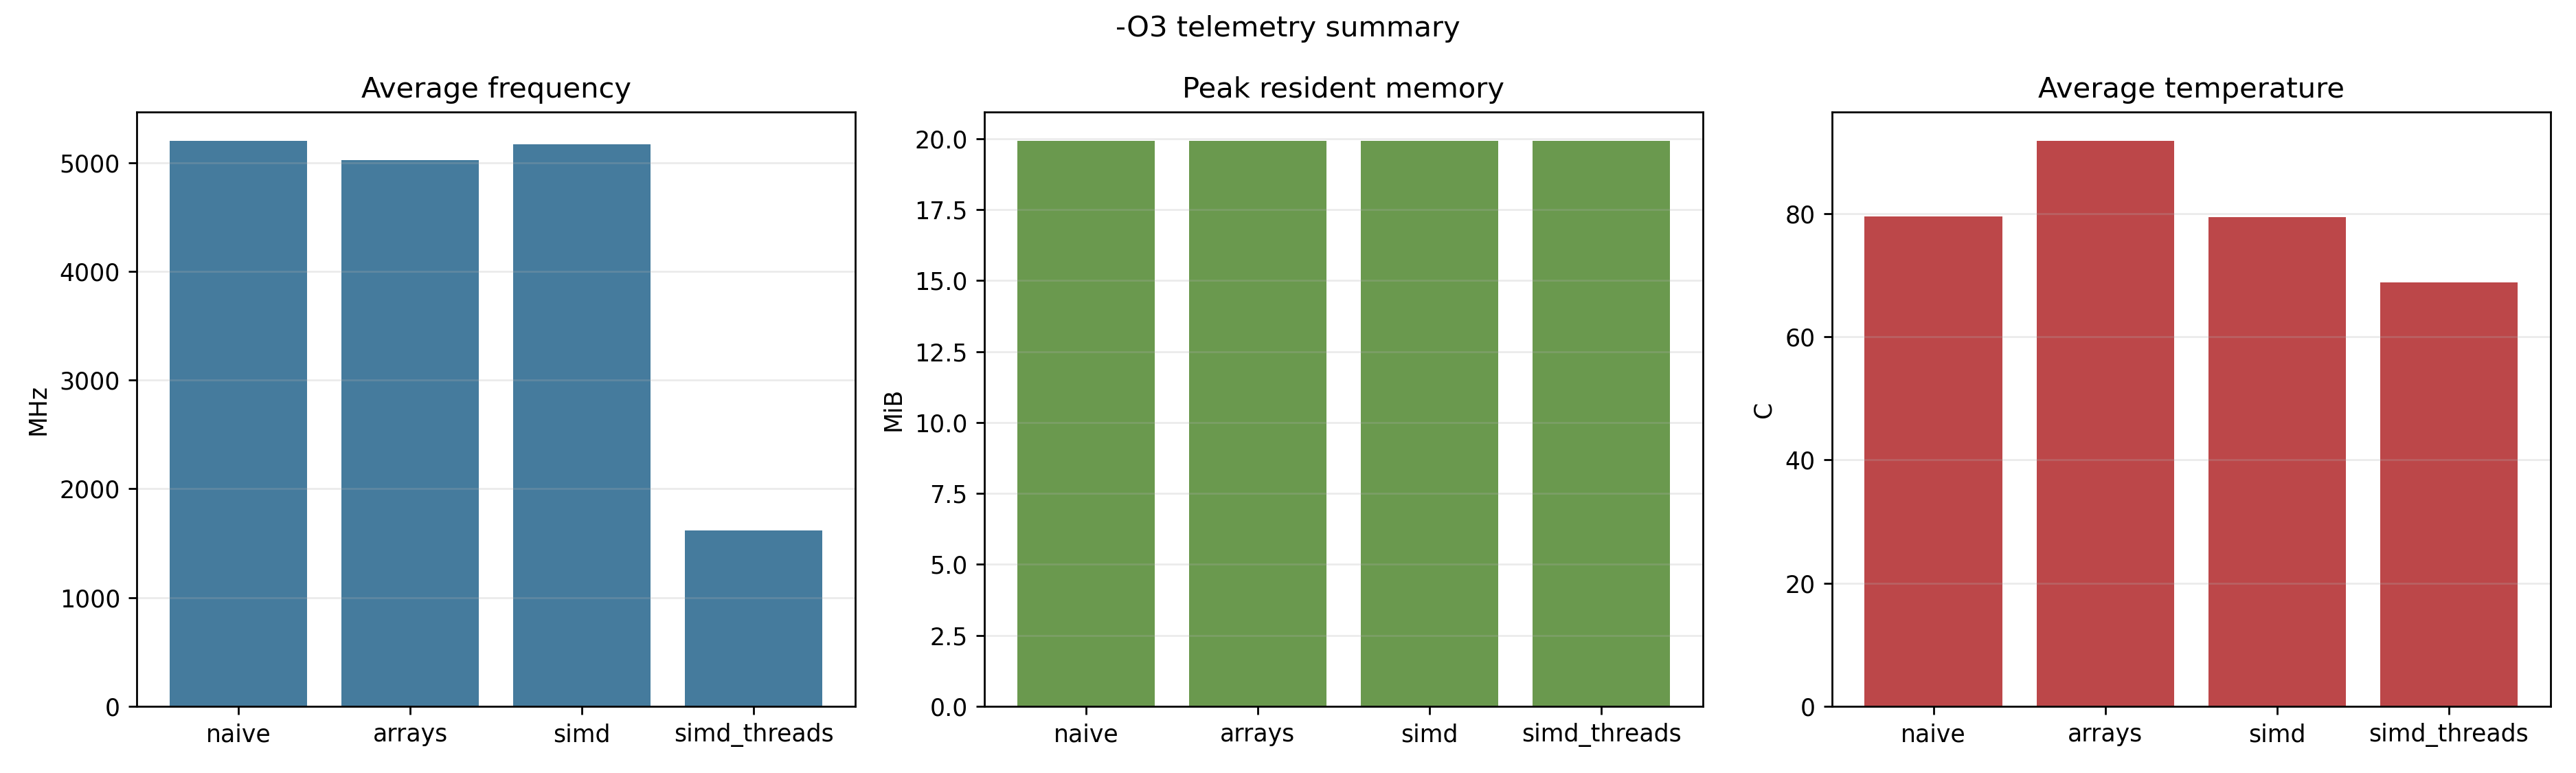
\includegraphics[width=0.95\linewidth]{../img/plots/benchmark_o3_telemetry.png}
\end{figure}

\begin{figure}[H]
\centering
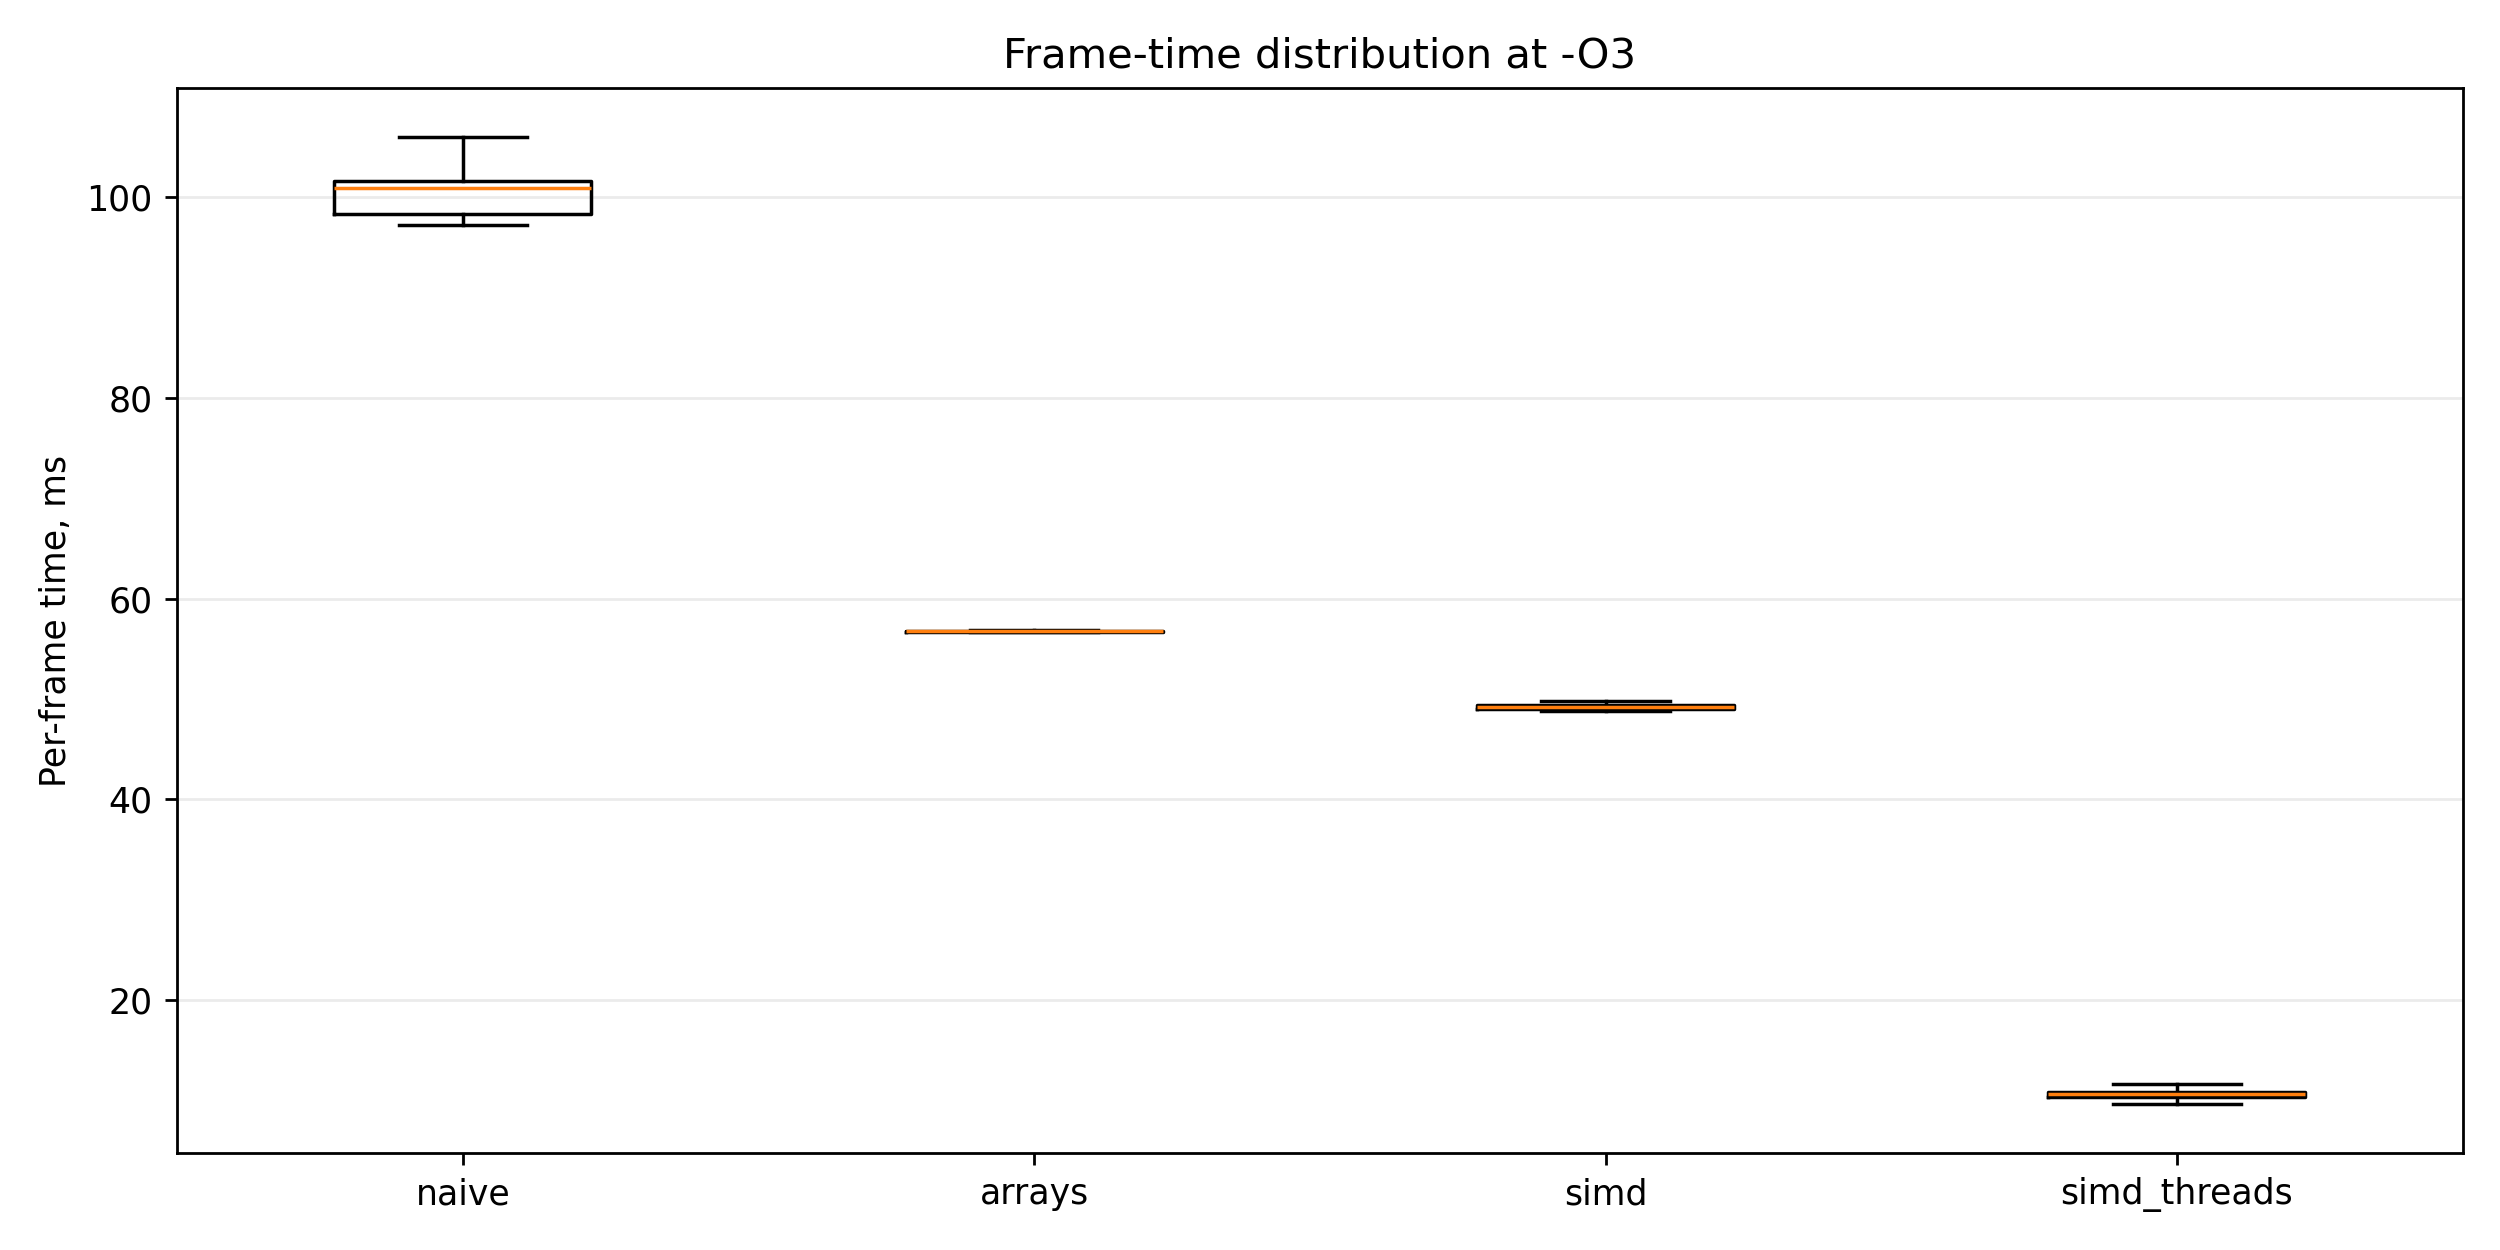
\includegraphics[width=0.95\linewidth]{../img/plots/benchmark_o3_boxplot.png}
\end{figure}

\begin{figure}[H]
\centering
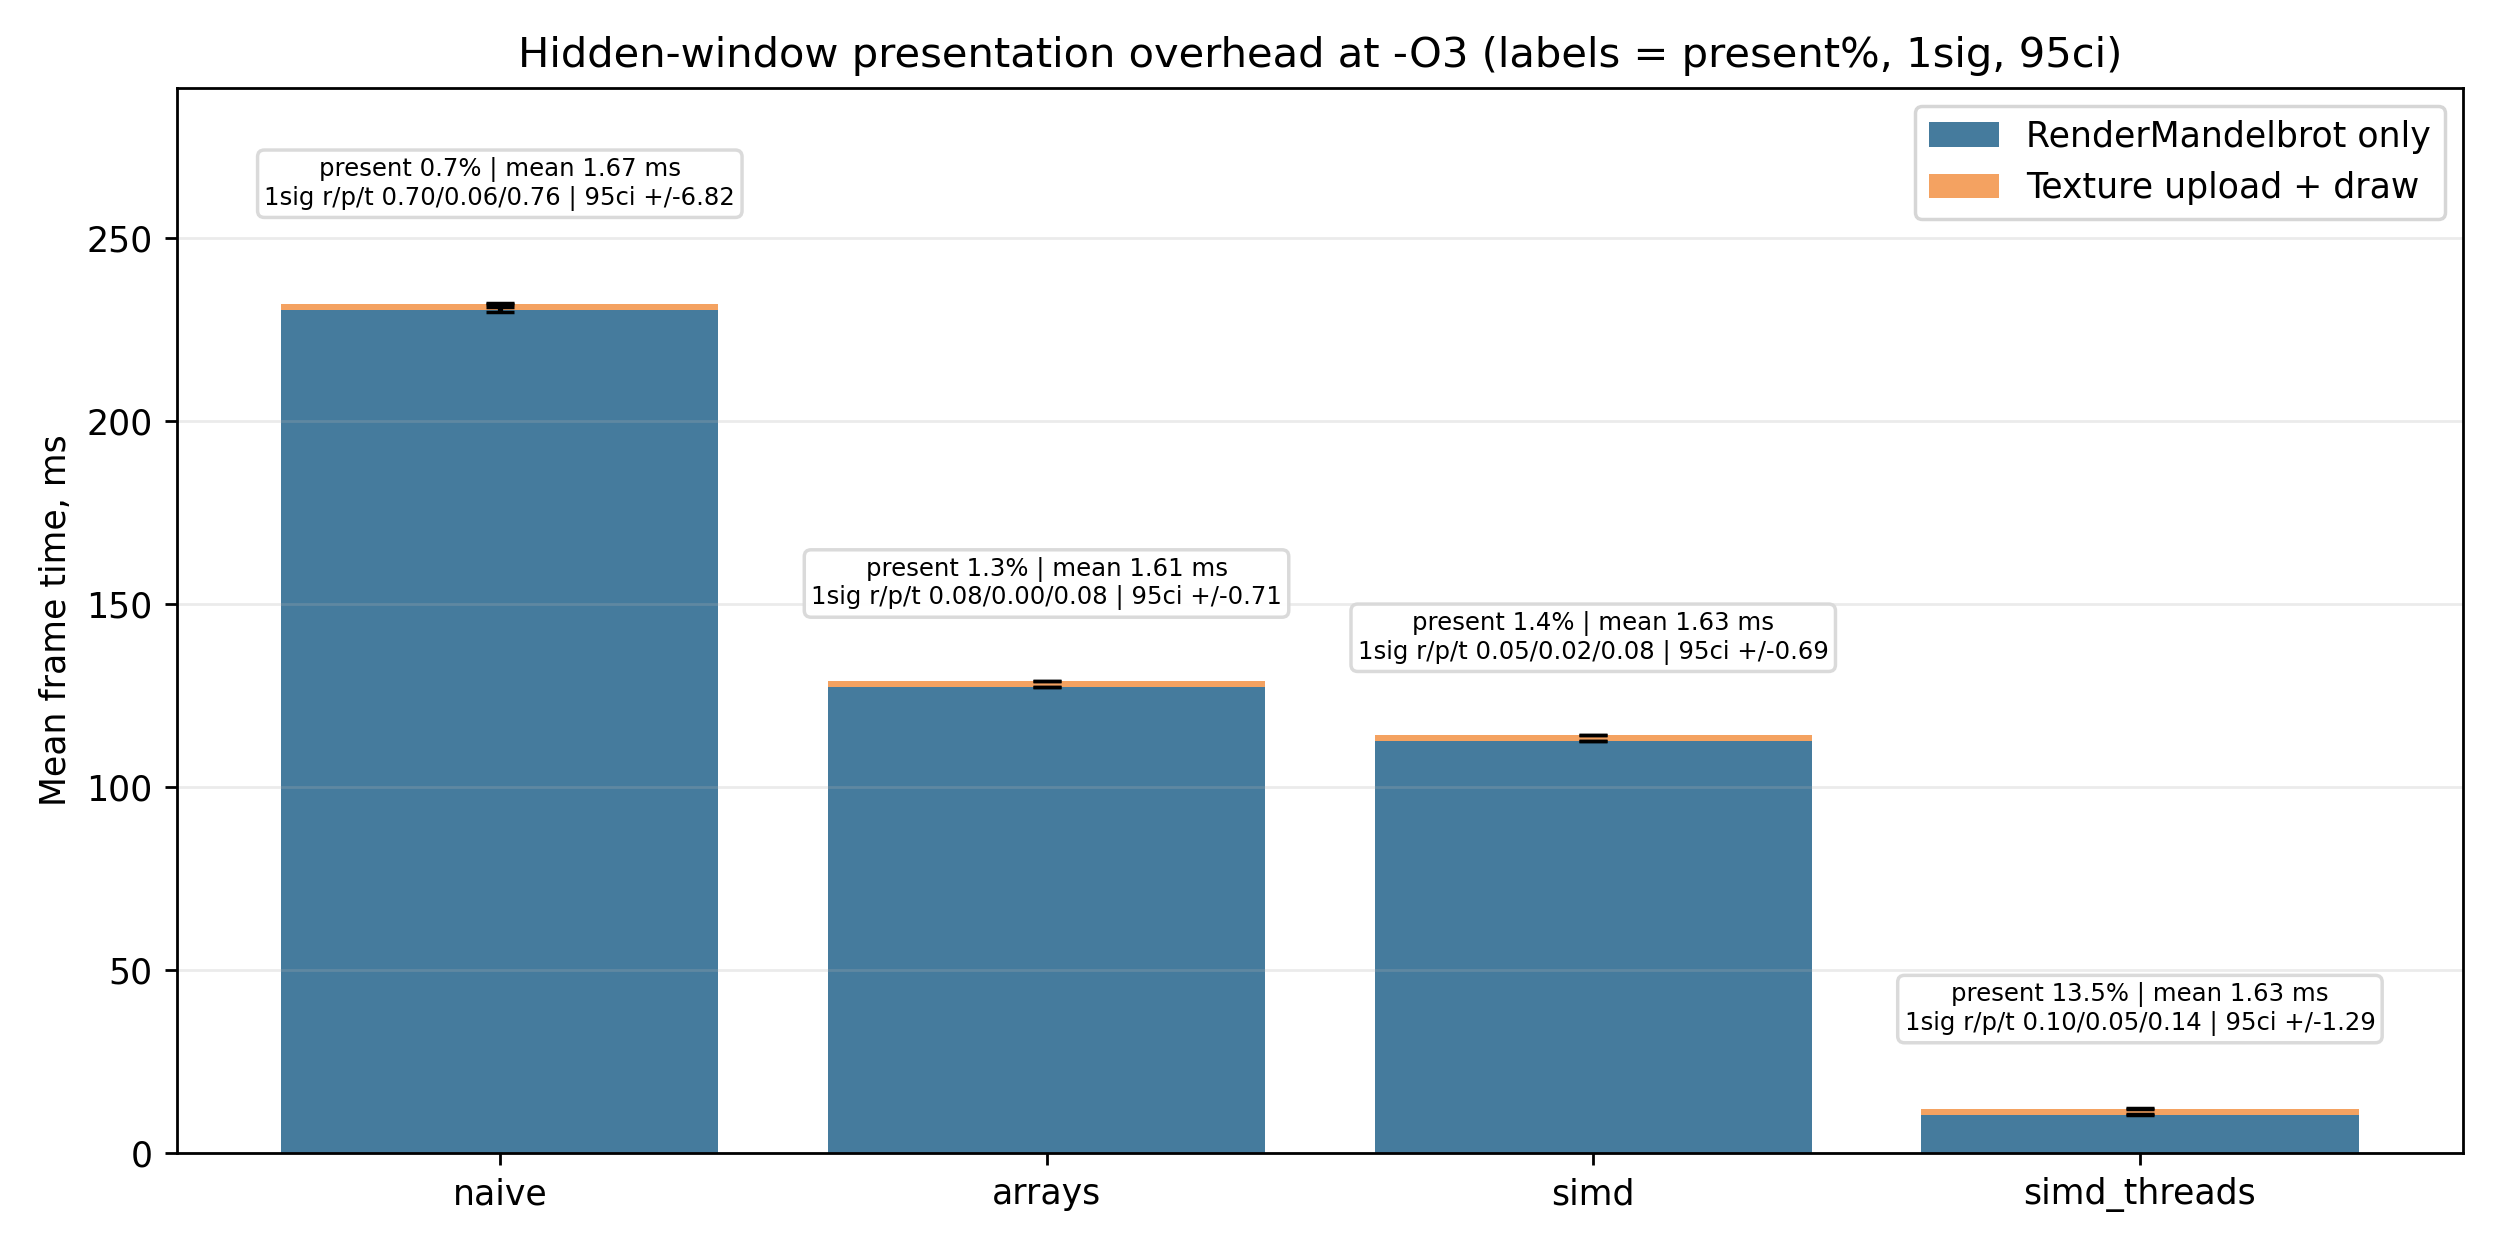
\includegraphics[width=0.95\linewidth]{../img/plots/benchmark_present_overhead.png}
\end{figure}

\begin{figure}[H]
\centering
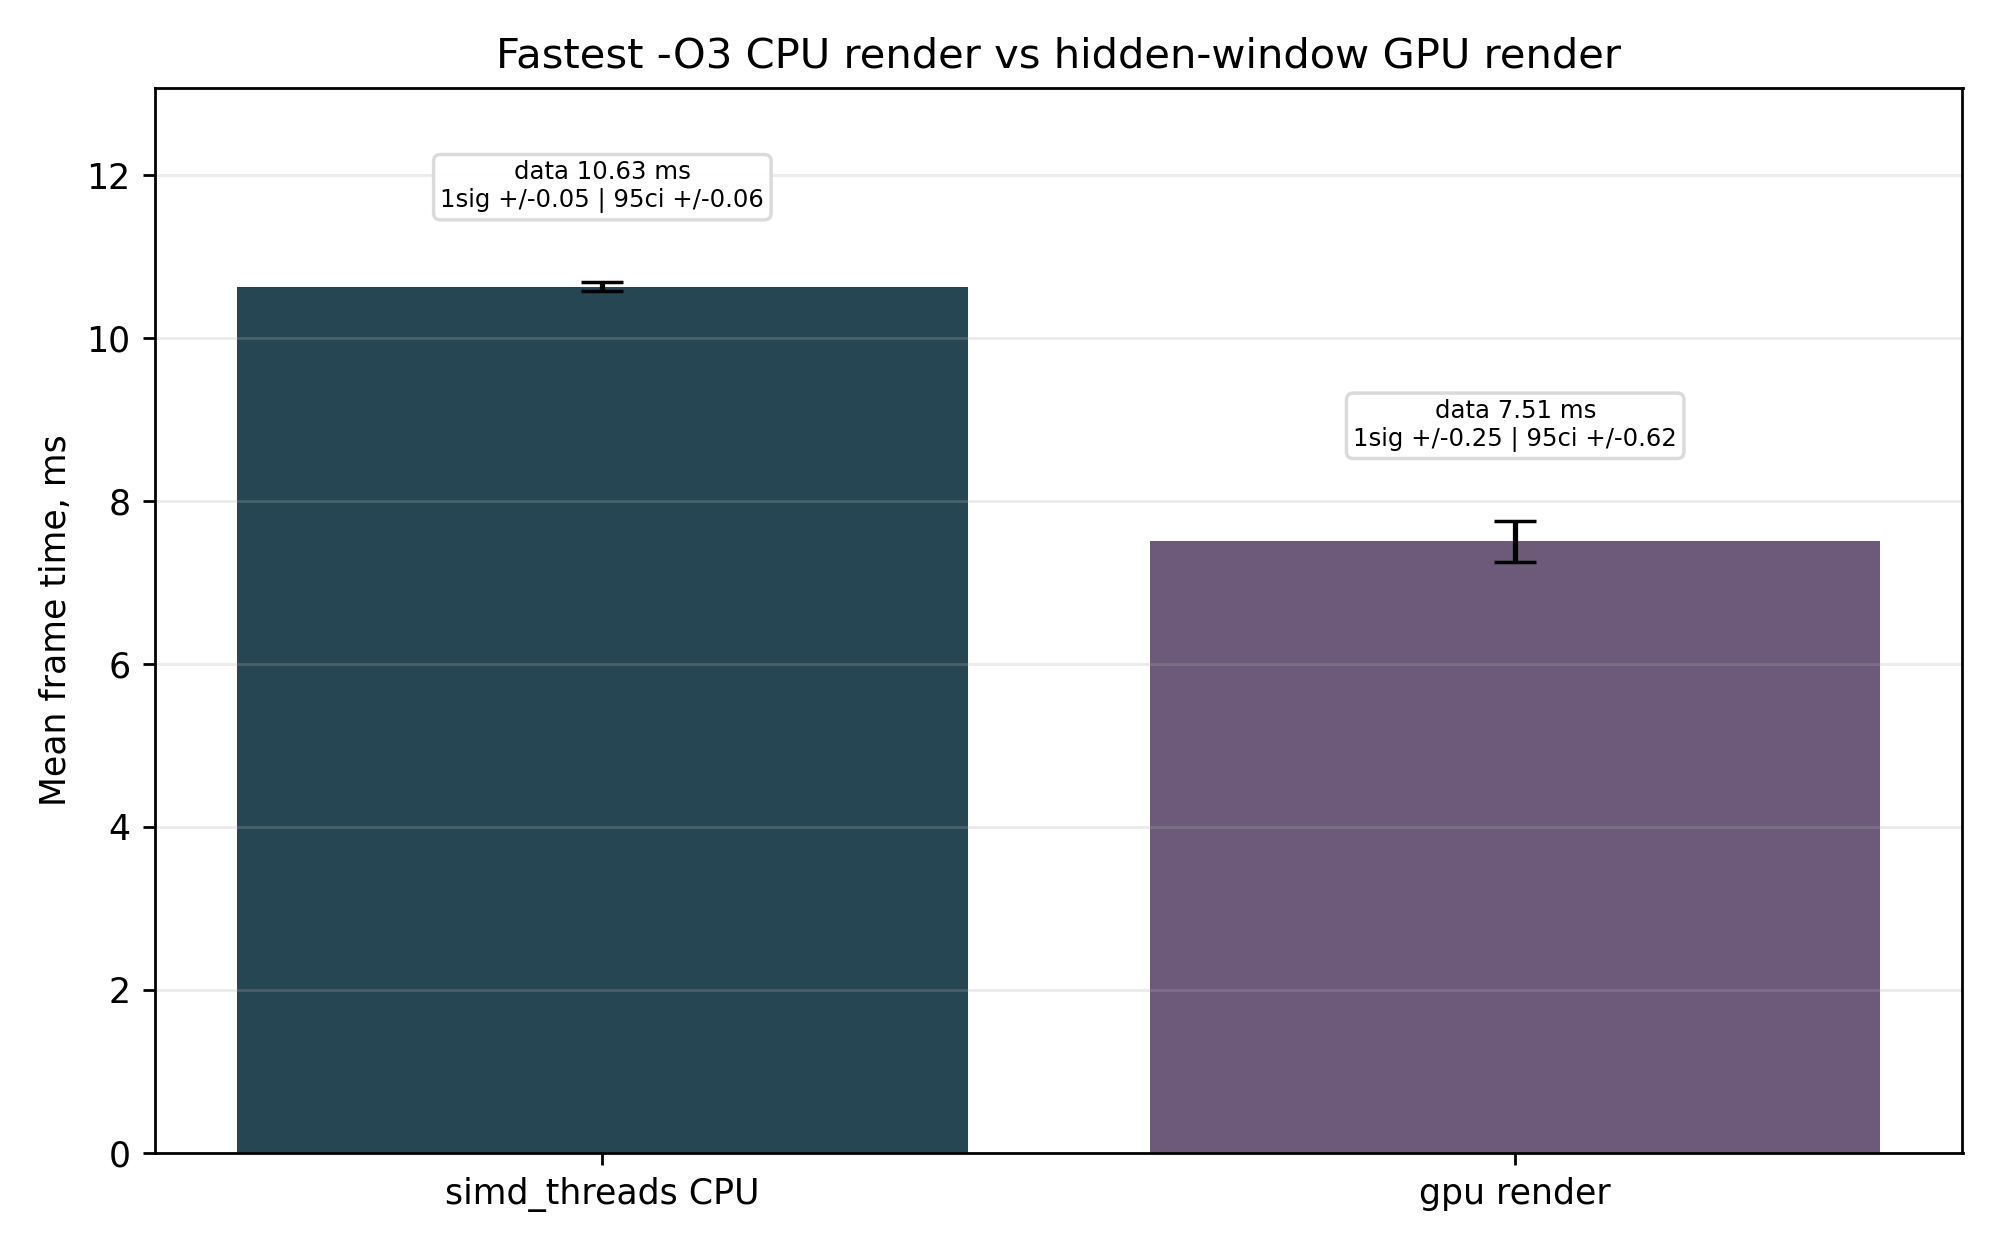
\includegraphics[width=0.95\linewidth]{../img/plots/benchmark_gpu_vs_cpu.png}
\end{figure}


\end{document}
